\section{Event Selections} \label{section:higgs_selections}
For the purpose of reconstruction of physics objects of interest, CMS utilizes Particle Flow Algorithm~\cite{CMS-PAS-PFT-10-002}, which aims to identify individual final state particles: photons, electrons, various hadrons, muons, etc. The main idea behind this algorithm is to use information not just from a particular subsystem (Muon, HCAL, ECAL, Tracker), but to combine and cross-reference features from various subdetectors: hits in the Tracker with Muon Stations, or clusters of energy depositions in ECAL, etc. In other words, this is an example of a sophisticated clusterization technique aimed to improve the reconstruction efficiency.

%For the purpose of our search, given the potential final states, the most important physics objects to be used are muons and jets. On top,

\subsection{Muon Selections}
The muon candidates are reconstructed using the Particle Flow Algorithm by matching compatible track segments from the inner silicon tracker and the muon detectors~\cite{Chatrchyan:2012xi}. In our analysis, we require only muons within the pseudorapidity range $|\eta|<2.4$ and with a minimum transverse momentum $p_{T}>10$ GeV. Furthermore, we require our muon to have $\Delta \beta$-corrected relative isolation, defined in equation~\ref{eq:higgs_selections_isolation}, of $I_{rel}^{PF}<0.25$. In the definition of the isolation variable $p_{T}^{ch}$ is the charged hadron transverse momenta sum, $E_{T}^{\gamma}$ is the photon transverse energy sum, and $E_{T}^{nh}$ is the neutral hadron transverse energy sum. The term $p_{T}^{chPU}$ is the estimated transverse momentum of charged particles from pileup in the $\Delta R < 0.4$, defined in equation~\ref{eq:higgs_selections_deltar}, cone, and the factor of 0.5 is used to estimate the neutral pileup from the charged component.
\begin{center}
   \begin{equation}
      \label{eq:higgs_selections_deltar}
      {\Delta R} = {\sqrt{\Delta\eta^{2}+\Delta\phi^{2}}}
   \end{equation}
\end{center}
\begin{center}
   \begin{equation}
      \label{eq:higgs_selections_isolation}
      {I_{rel}^{PF}} = {(p_{T}^{ch}+max(0,E_{T}^{\gamma}+E_{T}^{nh}-0.5*p_{T}^{chPU}))/p_{T}^{\mu}}
   \end{equation}
\end{center}

Additionally, we only utilize ``Medium Id'' muons provided and recommended centrally by the CMS Physics Object Group~\cite{CMSMuonPOG,CMSMuonId}. As we mentioned previously, muons are reconstructed using clusters of hits from various subsystems (Tracker and Muon Stations); in other words we define a physics object Muon to be a composite cluster of combined hits from Tracker and Muon Systems. It's important to understand the difference between actual particles Muons and our definition of a muon! Moreover, when extracting the momentum of a muon, a certain regression procedure is performed, a fit for instance, from which we can extract the goodness of fit or some other quality metric, using which we can judge upon the quality of the reconstructed candidate. Finally, Muon Id is a set of criteria that define a muon candidate of certain quality and allow us to discriminate candidates based on this feature.

\subsection{Muon Corrections}
Given a very narrow theoretical width of the Higgs Boson, $4.2$ MeV, the Higgs peak is dominated by the Muon detector resolution which is on the order of several GeV. Therefore, to increase the sensitivity of our search, it's crucial to have the best possible dimuon mass resolution, both in data and Monte Carlo. Moreover, as it is going to be described further in the Statistical Modeling sections, we need to correct for possible dimuon mass scale shifts.

There are two different sets of Muon corrections tested: Rochester~\cite{CMSRochesterCorrections} and Kalman~\cite{CMSKalmanCorrections}. Both allow to correct the scale and smear the resolution. For the validation purposes, we look at the Z peak scale and resolution using these two sets. In Figures~\ref{fig:higgs_selections_zscale}, ~\ref{fig:higgs_selections_zresolution}  comparisons of uncorrected with the two types of corrections are shown for the scale and resolution, respectively. Both the Rochester and Kalman muon corrections successfully align Data with MC in terms of the Z peak.
\begin{figure}[hbp]
  \centering
  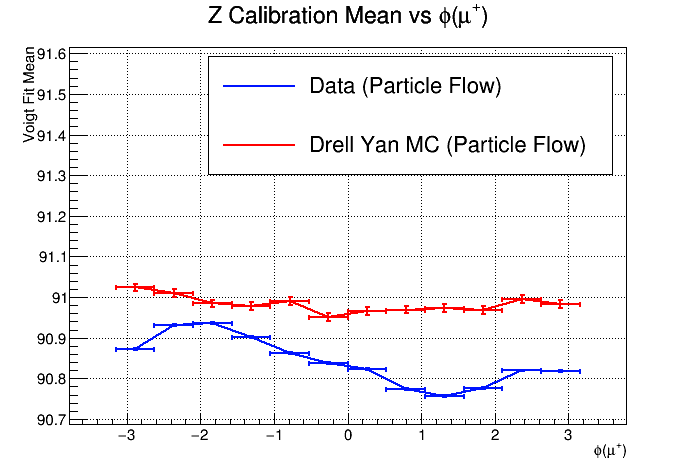
\includegraphics[width=0.32\linewidth]{figures/muon_calib/zcal_pf_mc-data_mean_phi_plus.png}
  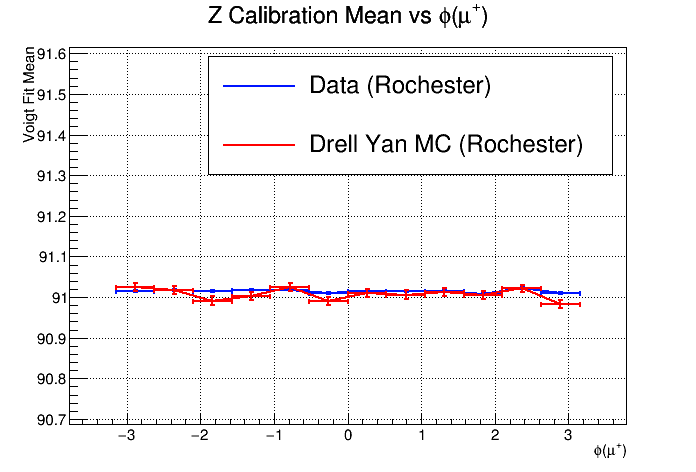
\includegraphics[width=0.32\linewidth]{figures/muon_calib/zcal_roch_mc-data_mean_phi_plus.png}
  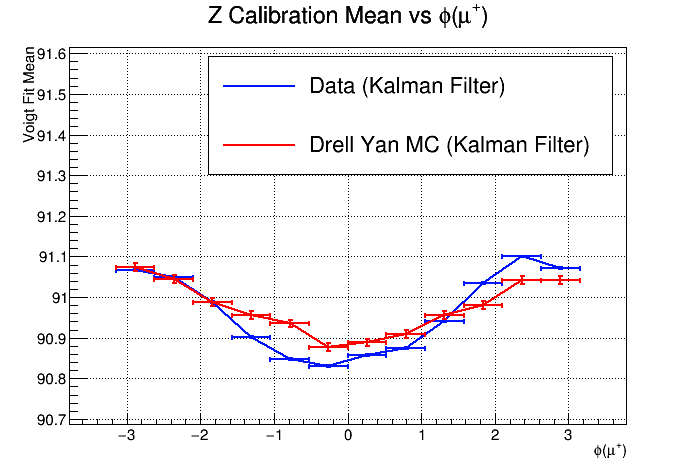
\includegraphics[width=0.32\linewidth]{figures/muon_calib/zcal_kamu_mc-data_mean_phi_plus.png}\\
  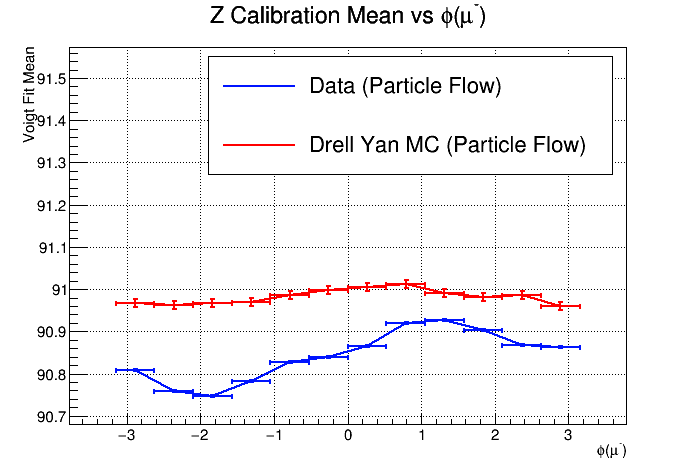
\includegraphics[width=0.32\linewidth]{figures/muon_calib/zcal_pf_mc-data_mean_phi_minus.png}
  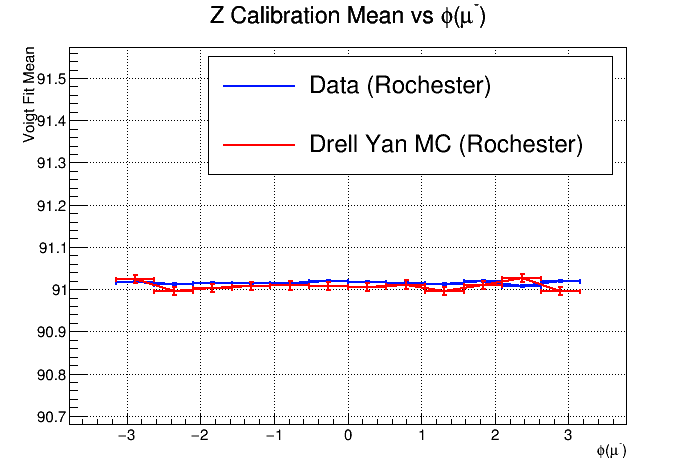
\includegraphics[width=0.32\linewidth]{figures/muon_calib/zcal_roch_mc-data_mean_phi_minus.png}
  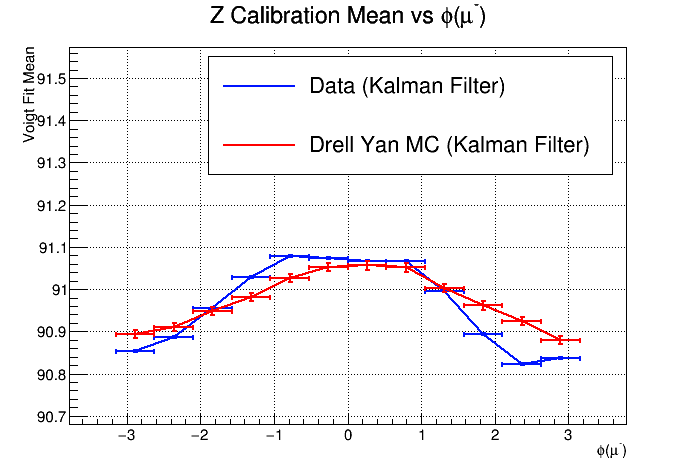
\includegraphics[width=0.32\linewidth]{figures/muon_calib/zcal_kamu_mc-data_mean_phi_minus.png}
  \caption{Comparing Uncorrected (left), Rochester (center) and Kalman (right) Corrections effects on Z Scale.}
  \label{fig:higgs_selections_zscale}
\end{figure}

\begin{figure}[hbp]
  \centering
  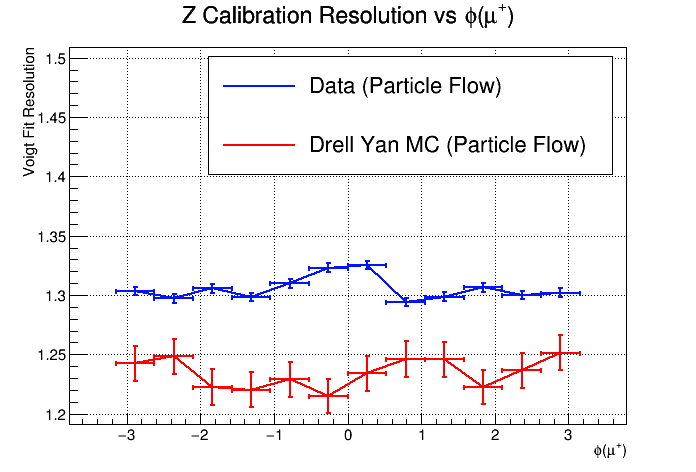
\includegraphics[width=0.32\linewidth]{figures/muon_calib/zcal_pf_mc-data_res_phi_plus.png}
  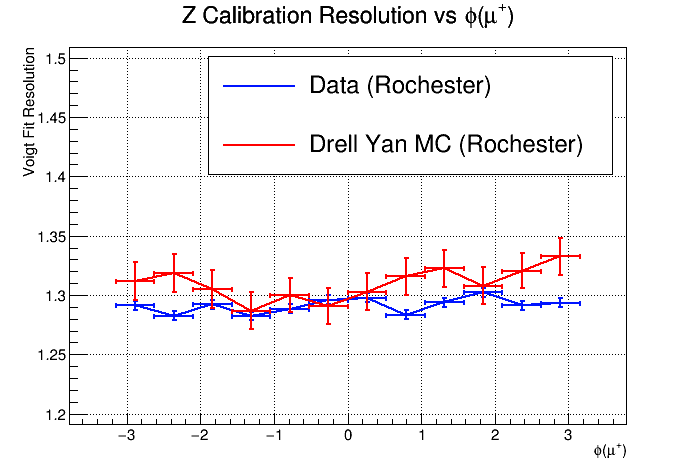
\includegraphics[width=0.32\linewidth]{figures/muon_calib/zcal_roch_mc-data_res_phi_plus.png}
  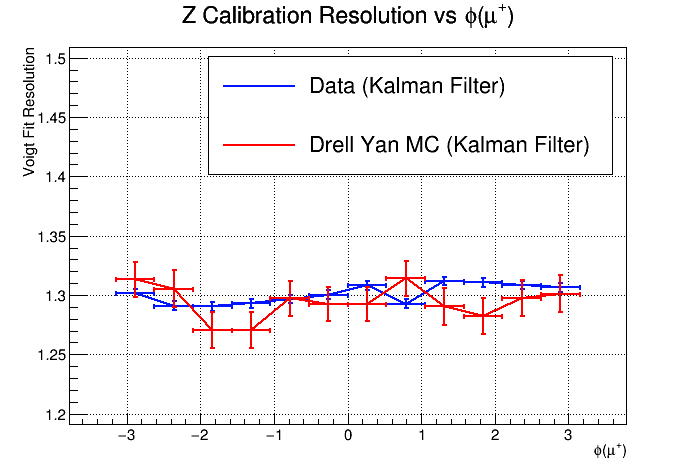
\includegraphics[width=0.32\linewidth]{figures/muon_calib/zcal_kamu_mc-data_res_phi_plus.png}\\
  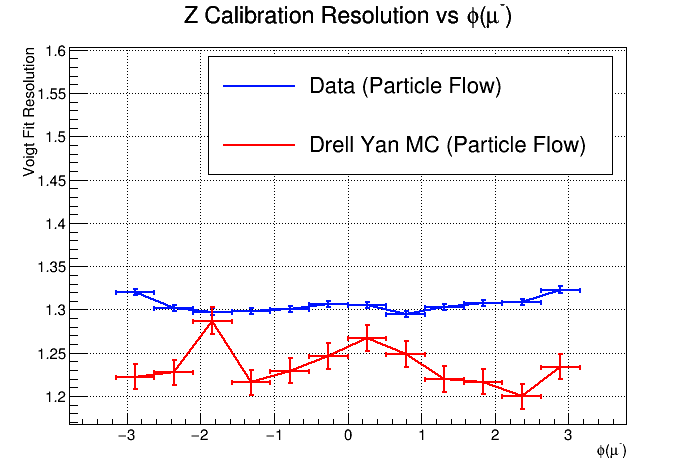
\includegraphics[width=0.32\linewidth]{figures/muon_calib/zcal_pf_mc-data_res_phi_minus.png}
  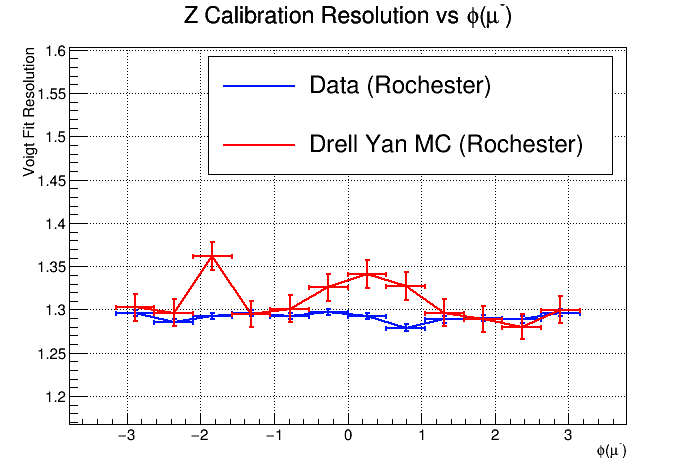
\includegraphics[width=0.32\linewidth]{figures/muon_calib/zcal_roch_mc-data_res_phi_minus.png}
  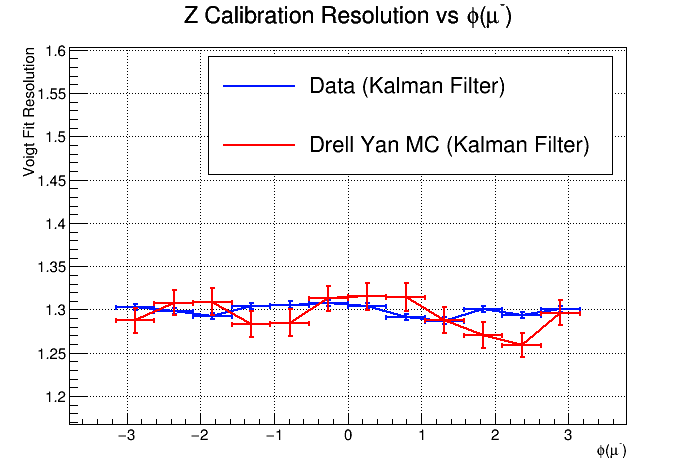
\includegraphics[width=0.32\linewidth]{figures/muon_calib/zcal_kamu_mc-data_res_phi_minus.png}
  \caption{Comparing Uncorrected (left), Rochester (center) and Kalman (right) Corrections effects on Z Resolution.}
  \label{fig:higgs_selections_zresolution}
\end{figure}

\subsection{Jet Selections}
Jets are reconstructed from PF candidates with the anti-$\kappa_{T}$ algorithm~\cite{Cacciari:2008gp} with a distance parameter of 0.4 after rejecting the charged hadrons that are associated to pileup primary vertices. Jets are cleaned against muons - jets overlapping with the selected PF muons, $\Delta R < 0.4$, are not considered further in the analysis. The selected jets with a minimum \pt of 30 GeV and a maximum $|\eta|$ of 4.7 are corrected in energy in order to account for the non-uniform detector response.

The PF jets are further required to fulfill the jet identification criteria.
Candidates with $|\eta|$ less than 2.7 are required to contain at
least one charged PF candidate and have a non-zero charged energy fraction,
and a charged electromagnetic energy fraction less than 0.99. The
neutral and photon energy fraction must be less than 0.99. Jets in
the region $2.7<|\eta|<3.0$ are required to have a neutral electromagnetic
fraction of greater than 0.01 and neutral hadron fraction less than
0.98 while jets with pseudorapidity above 3.0 are required to have more
than 10 neutral particles and a neutral electromagnetic energy fraction
less than 0.9.

For reconstructed jets with $|\eta| < 2.4$, the combined secondary vertex b-tagging algorithm (CSVv2)~\cite{Chatrchyan:2012jua} response is used to discriminate against the $t\bar{t}$ background process events when defining the event categories. The CSVv2 medium operating point is chosen as base line for this analysis and corresponds to a b-tagging efficiency of $60-65\%$ while the misidentification rate for light quarks such as $u$, $d$, $s$, and gluon jets is approximately 1\%.

\subsection{HLT Selections}
Our search requires one of the following Single Isolated Muon Triggers to fire per event:
\begin{itemize}
  \item HLT\_IsoMu24
  \item HLT\_IsoTkMu24
\end{itemize}
The choice of the threshold is driven by the requirement of the lowest \pt threshold to be present during the whole course of datataking. These triggers require the event to have at least one isolated muon candidate with \pt above 24 GeV, with no explicit restriction on its pseudorapidity.

\subsection{Primary Vertex Selection}
One of the top requirements on selecting a proton-proton collision event is the presence of at least 1 valid Primary Vertex with the following conditions:
\begin{itemize}
  \item $ndf \ge 4$ - number of tracks originating from this PV is greater than 4
  \item $\rho < 2$ cm and $|Z| < 24$ cm - displacement along either Z-axis or in the transverse plan should be minimal w.r.t. Interaction Point, defined as (0,0,0).
\end{itemize}

\subsection{Selections Summary}
We can summarize cuts and selections for our search as follows:
\begin{itemize}
  \item At least 1 Primary Vertex passing the PV Selections
  \item At least 1 of the HLT Paths fired
  \item At least 2 opposite sign muons which pass Muon Selections. If more than 1 pair - choose the 2 candidates with the highest \pt. That is the Higgs Candidate.
  \item At least 1 muon from the Higgs Candidate pair with $p_t > 26$ GeV and is matched to the HLT Path that fires the event with $\Delta R < 0.1$.
  \item Filter out the jets that do not pass the Jet Selections, but do not require a certain number of them at this stage.
\end{itemize}

\subsection{Validation}
After applying all of the specified selections, we arrive at a set of events that we are going to further use in order to maximize the sensitivity of our search. However, before proceeding to the next section, we need to validate basic kinematic variables for the inclusive distributions.

First, in the figure~\ref{fig:higgs_selections_inclusivemassnocorr}, inclusive dimuon mass distribution is presented without any muon momentum corrections applied. Notice the presence of a kick near the Z peak. It is the result of a discrepancy in both the mass scale and resolution.
\begin{figure}[!h]
  \centering
  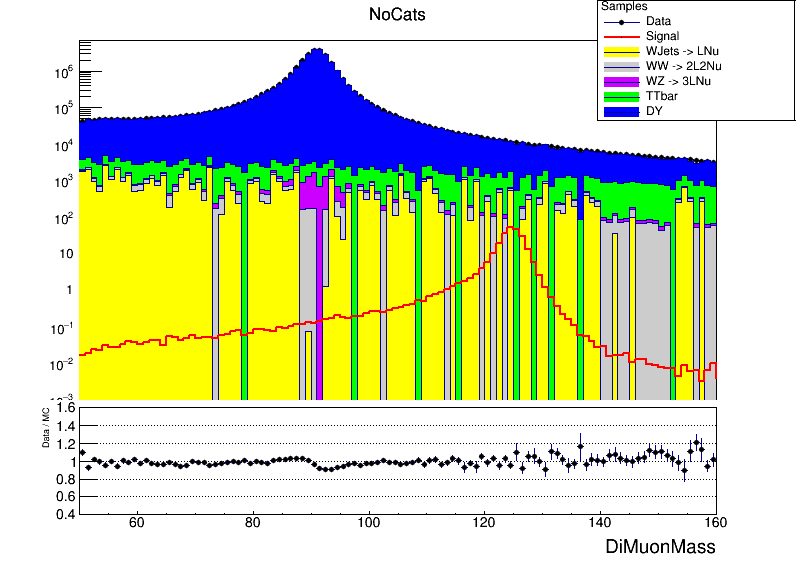
\includegraphics[width=0.5\linewidth]{figures/ch_higgs/distributions/baseline_nocorrections/distribution__NoCats__DiMuonMass__logY.png}
  \caption{Inclusive Dimuon Mass Distributions without any Muon Corrections. Notice the discrepancy around the Z peak}
  \label{fig:higgs_selections_inclusivemassnocorr}
\end{figure}

Second, in the figure~\ref{fig:higgs_selections_inclusivekinematic}, distributions of various kinematic variables after passing the selections are presented.
\begin{figure}[!h]
  \centering
  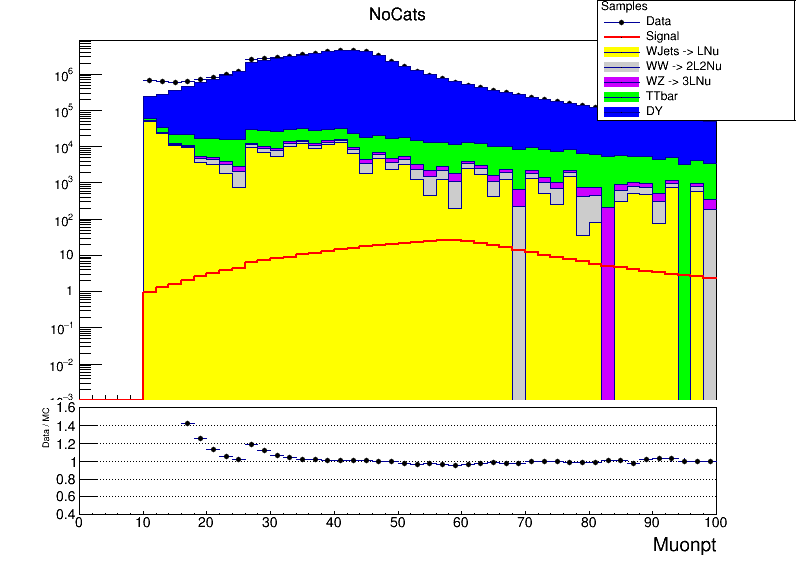
\includegraphics[width=0.45\linewidth]{figures/ch_higgs/distributions/baseline_kalman/distribution__NoCats__Muonpt__logY.png}
  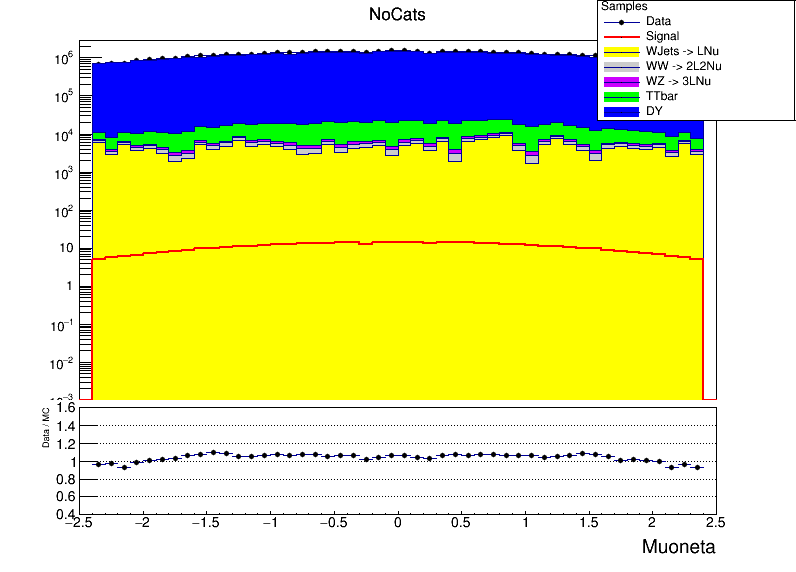
\includegraphics[width=0.45\linewidth]{figures/ch_higgs/distributions/baseline_kalman/distribution__NoCats__Muoneta__logY.png}\\
  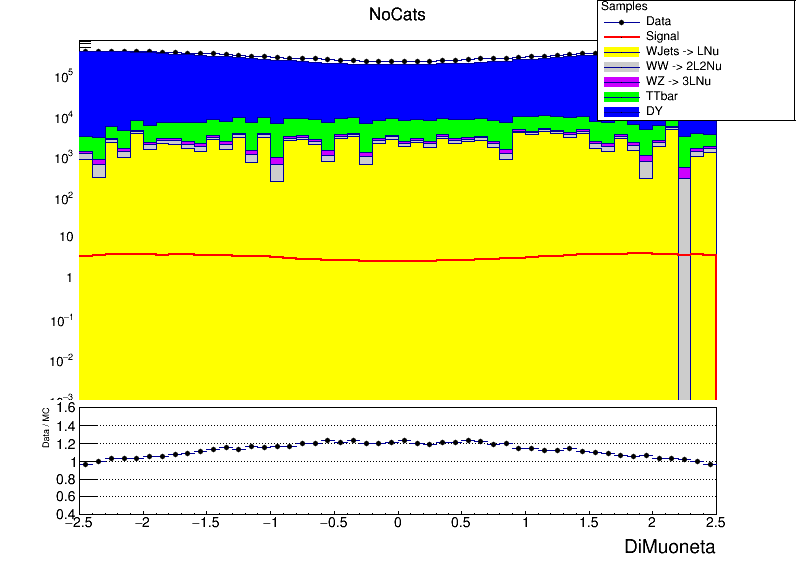
\includegraphics[width=0.45\linewidth]{figures/ch_higgs/distributions/baseline_kalman/distribution__NoCats__DiMuoneta__logY.png}
  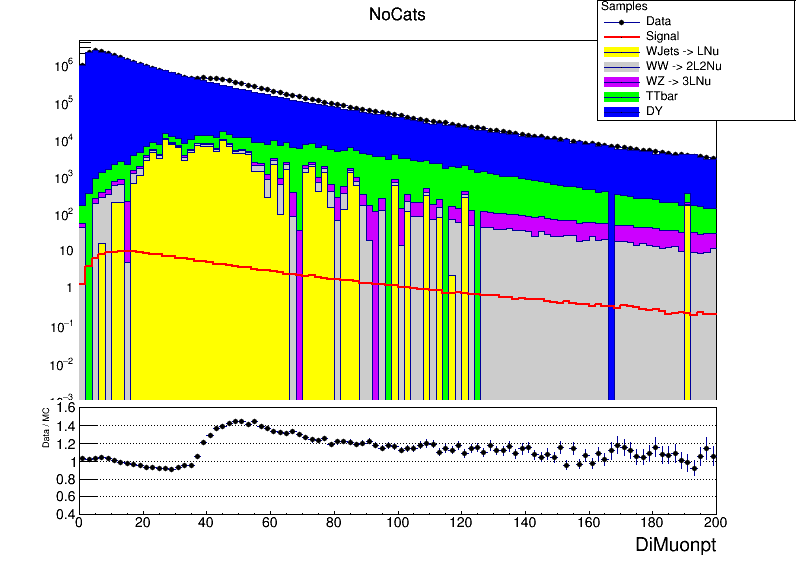
\includegraphics[width=0.45\linewidth]{figures/ch_higgs/distributions/baseline_kalman/distribution__NoCats__DiMuonpt__logY.png}
  \caption{Inclusive Kinematic Distributions.}
  \label{fig:higgs_selections_inclusivekinematic}
\end{figure}

Furthermore, in the figure~\ref{fig:higgs_selections_inclusivemass}, the inclusive dimuon mass distributions are shown with Rochester and Kalman corrections respectively applied to both Data and Monte Carlo. Notice that the discrepancy in scale and resolution is not present anymore around the Z peak.
\begin{figure}[hbp]
  \centering
  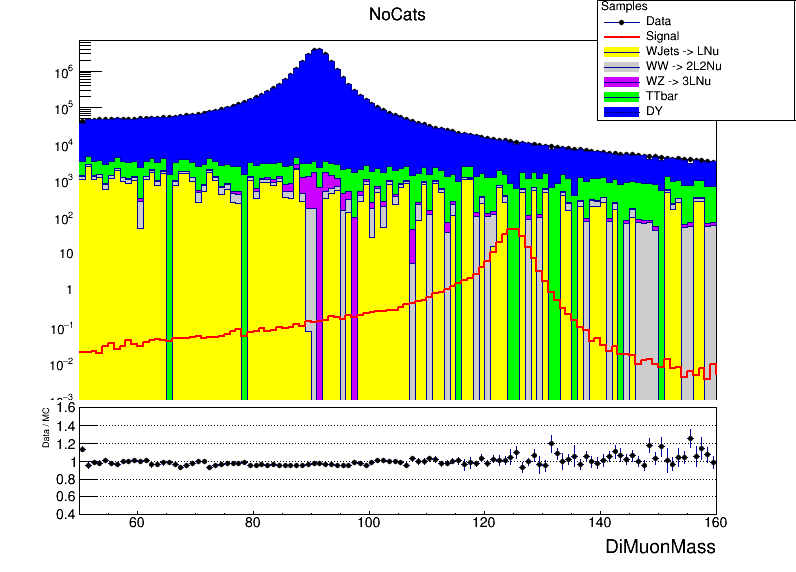
\includegraphics[width=0.9\linewidth]{figures/ch_higgs/distributions/baseline_rochester/distribution__NoCats__DiMuonMass__logY.png}\\
  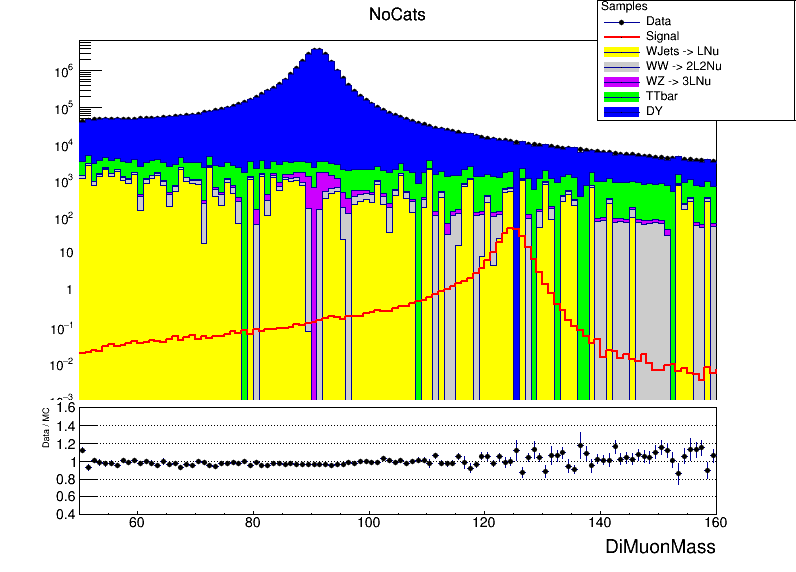
\includegraphics[width=0.9\linewidth]{figures/ch_higgs/distributions/baseline_kalman/distribution__NoCats__DiMuonMass__logY.png}
  \caption{Inclusive Dimuon Mass Distributions. Rochester (Left) and Kalman (Right) Corrections applied}
  \label{fig:higgs_selections_inclusivemass}
\end{figure}



% \subsection{Object validation}
% After applying all the selection cuts and scale factors, we validate the MC simulation
% on data events where the candidate muon pair has an invariant mass greater than 60~GeV.

% \begin{figure}[hbp]
%   \centering
%   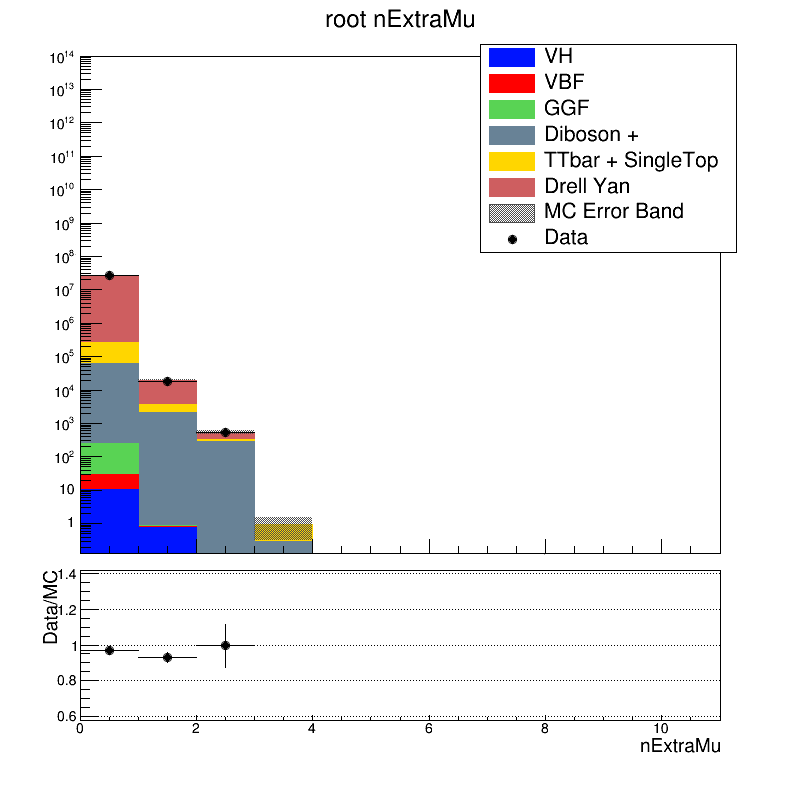
\includegraphics[width=0.32\linewidth]{figures/event_sel/nExtraMu_root.png}
%   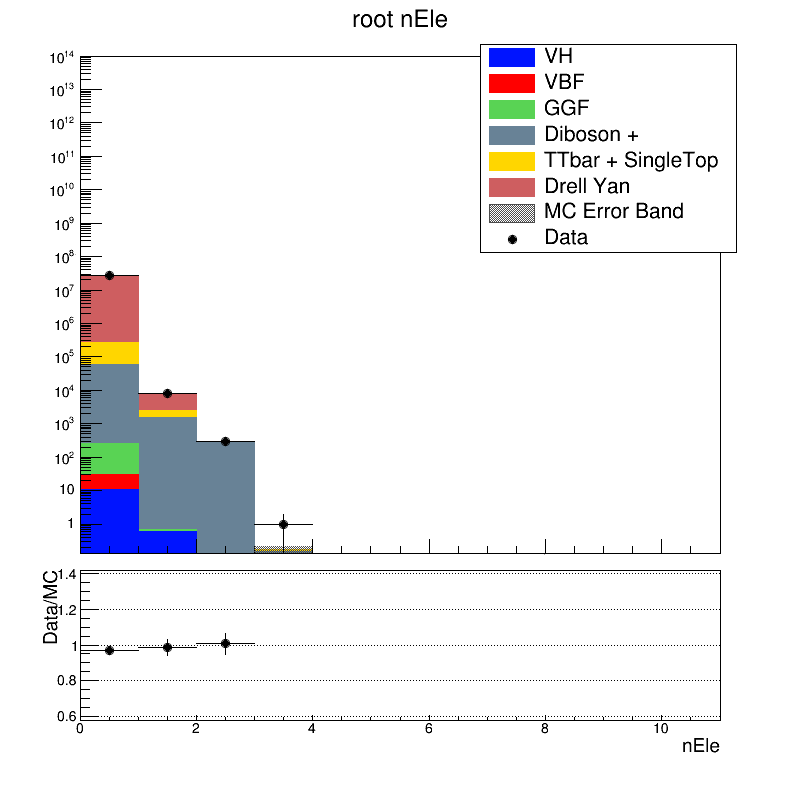
\includegraphics[width=0.32\linewidth]{figures/event_sel/nEle_root.png}
%   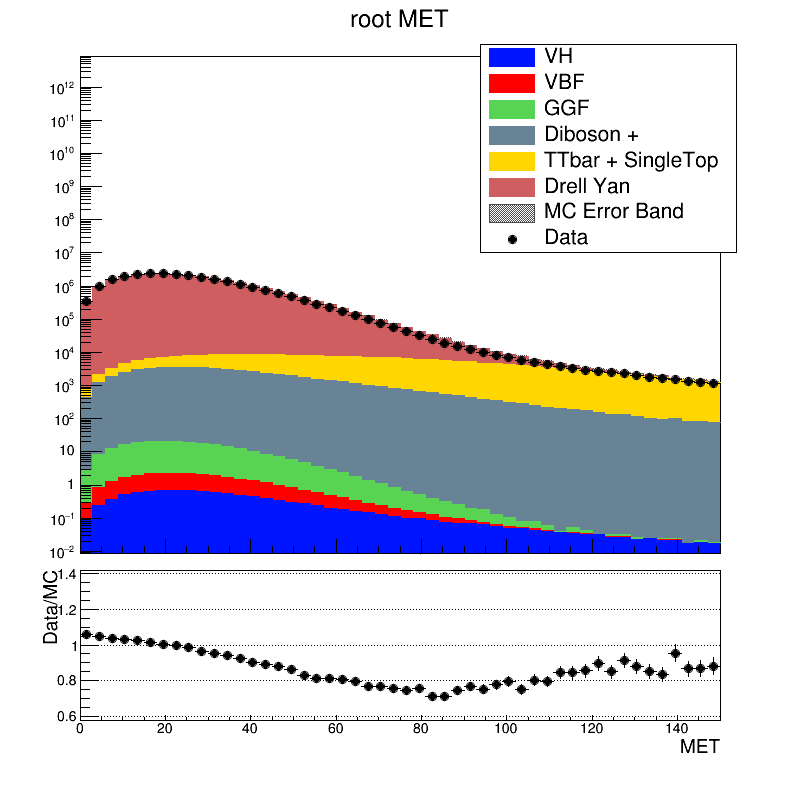
\includegraphics[width=0.32\linewidth]{figures/event_sel/MET_root.png}
%   \caption
%    {Validation of global event variables.}
%   \label{fig:valid_evt}
% \end{figure}

% \begin{figure}[hbp]
%   \centering
%   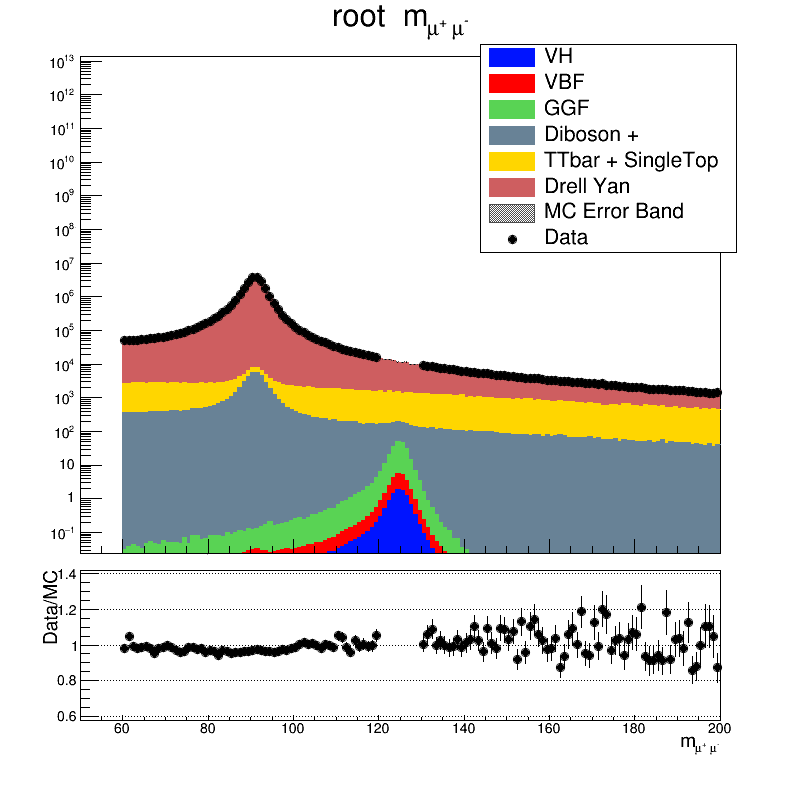
\includegraphics[width=0.32\linewidth]{figures/event_sel/dimu_mass_Roch_root.png}
%   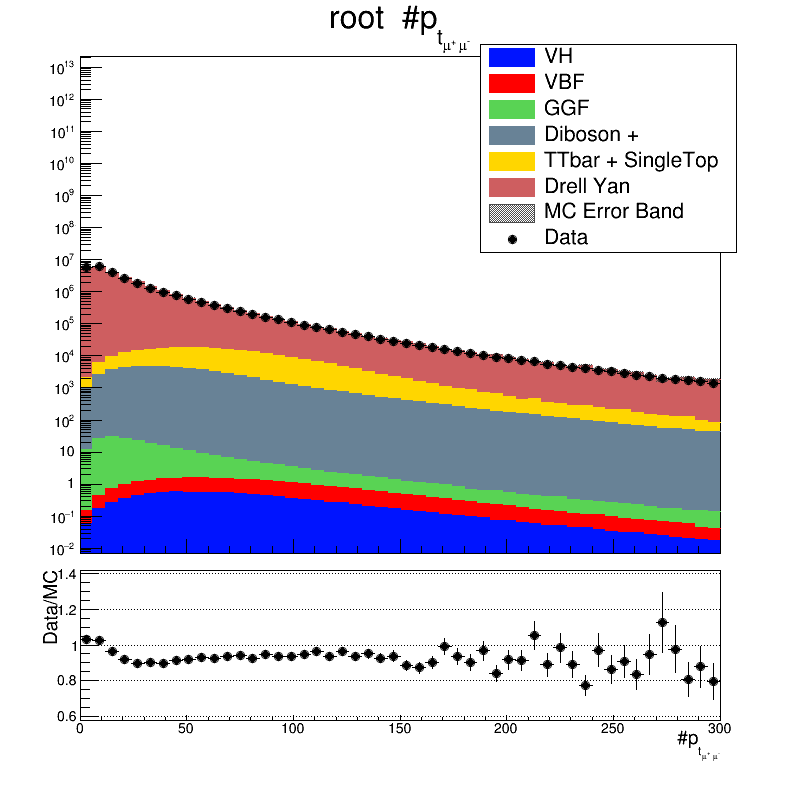
\includegraphics[width=0.32\linewidth]{figures/event_sel/dimu_pt_root.png}
%   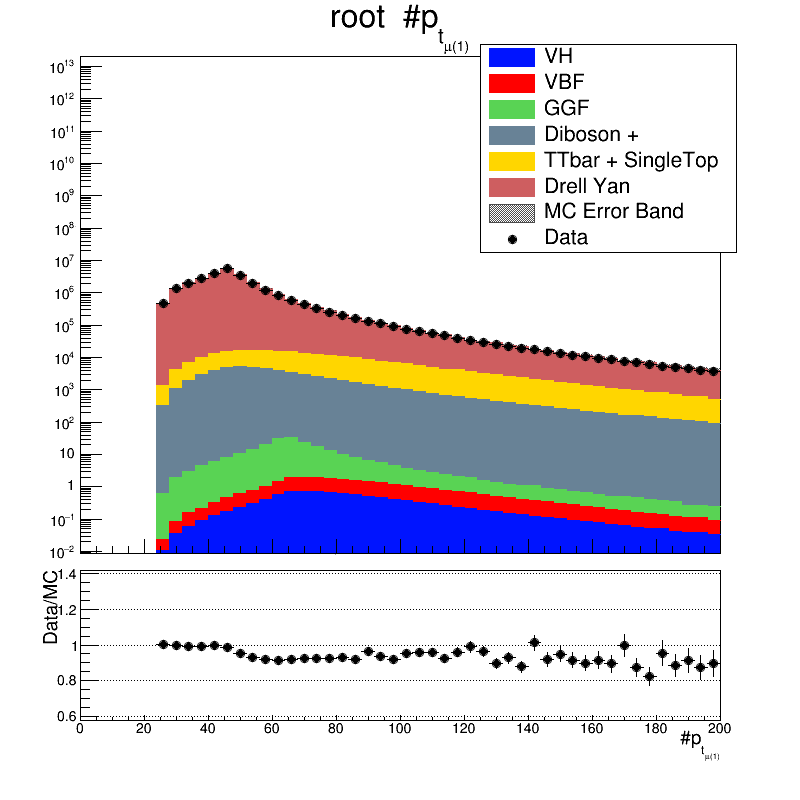
\includegraphics[width=0.32\linewidth]{figures/event_sel/mu1_pt_root.png}
%   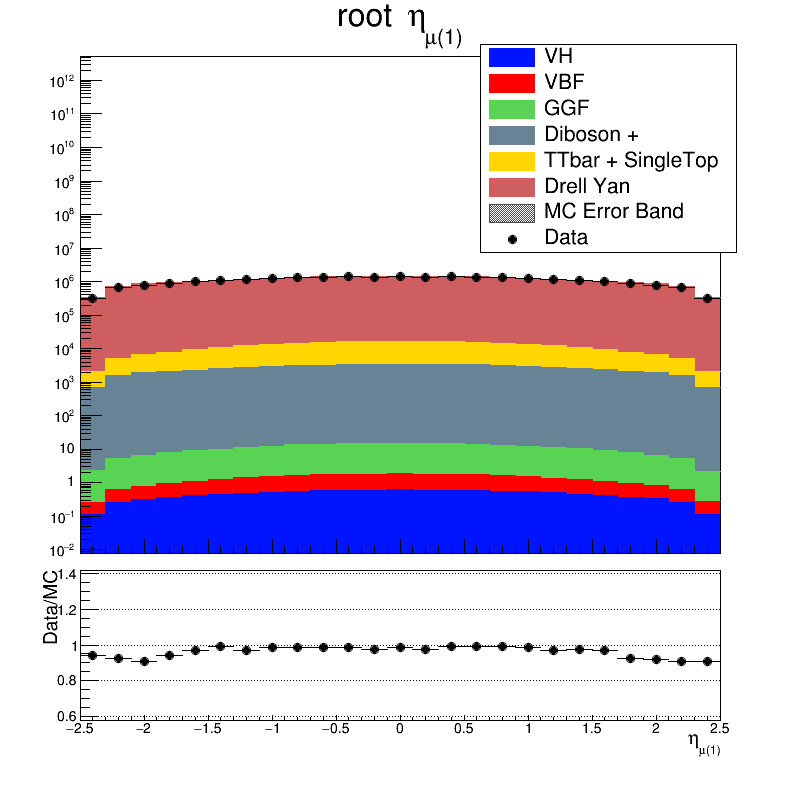
\includegraphics[width=0.32\linewidth]{figures/event_sel/mu1_eta_root.png}
%   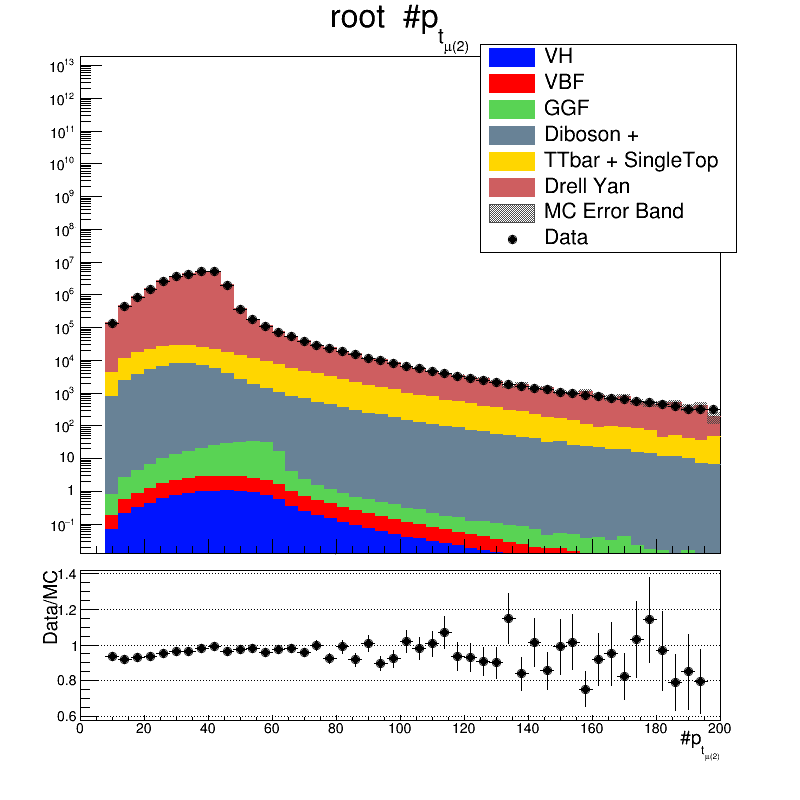
\includegraphics[width=0.32\linewidth]{figures/event_sel/mu2_pt_root.png}
%   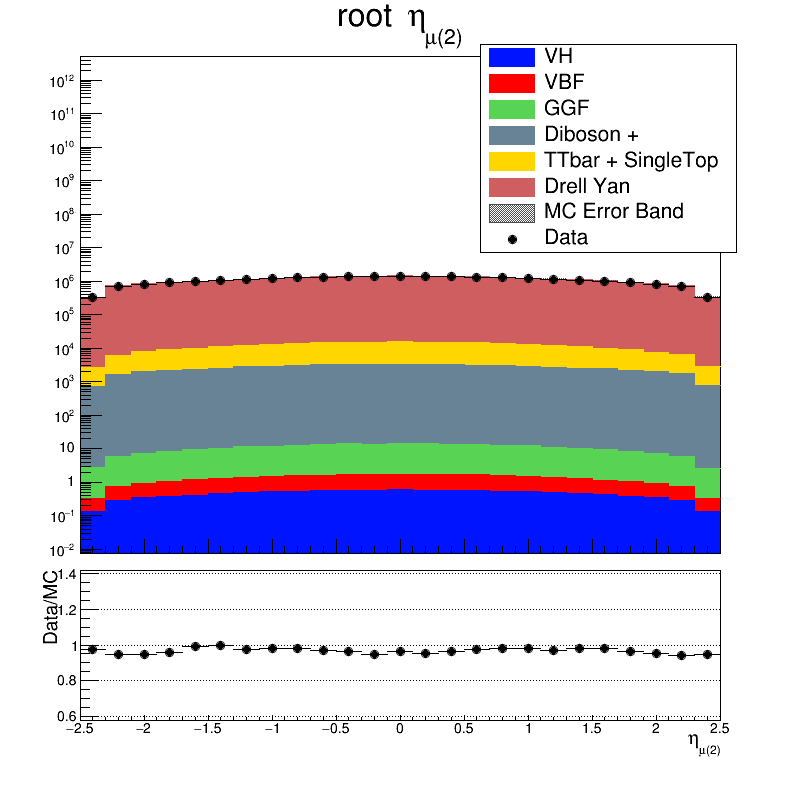
\includegraphics[width=0.32\linewidth]{figures/event_sel/mu2_eta_root.png}
%   \caption
%    {Validation of muon-related variables.}
%   \label{fig:valid_muons}
% \end{figure}

% \begin{figure}[hbp]
%   \centering
%   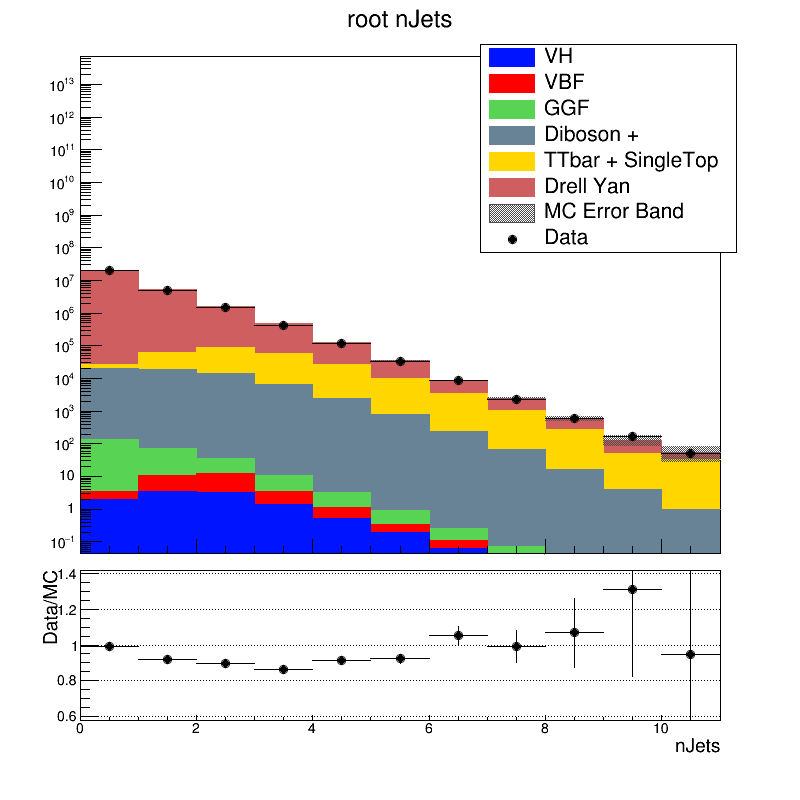
\includegraphics[width=0.32\linewidth]{figures/event_sel/nJets_root.png}
%   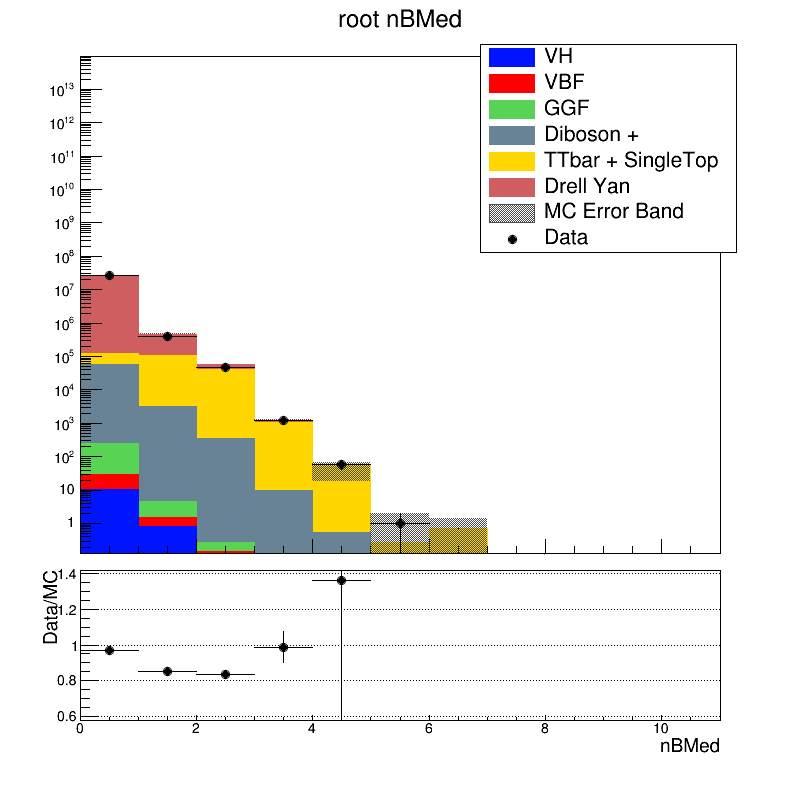
\includegraphics[width=0.32\linewidth]{figures/event_sel/nBMed_root.png}
%   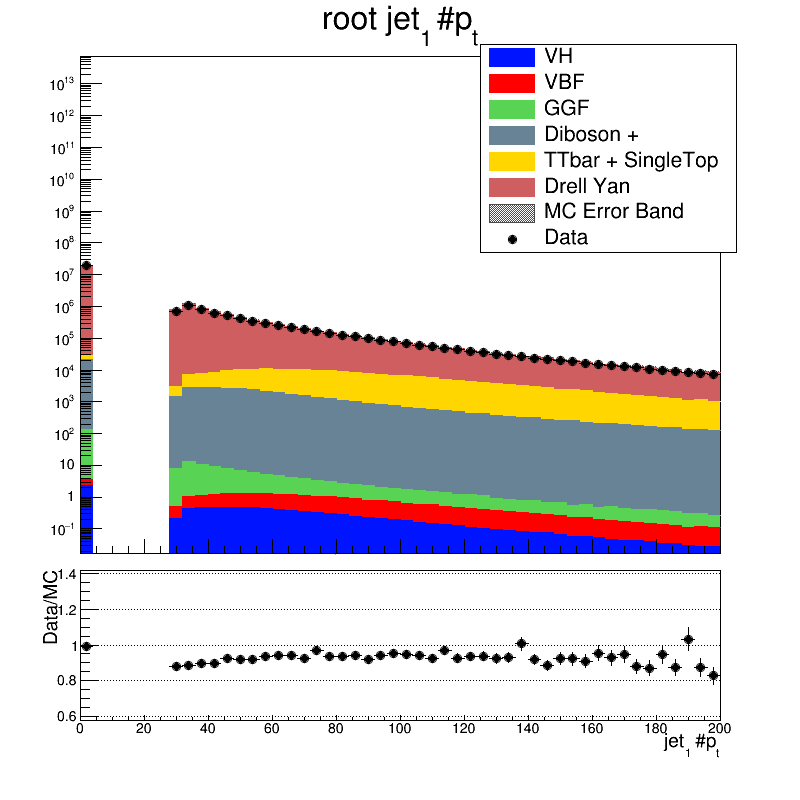
\includegraphics[width=0.32\linewidth]{figures/event_sel/jet1_pt_root.png}
%   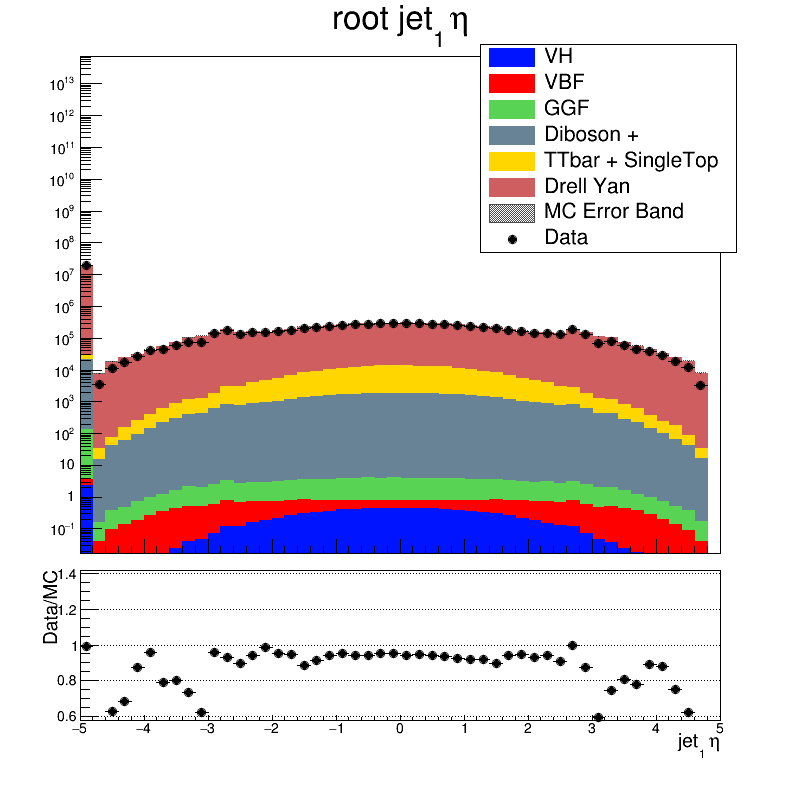
\includegraphics[width=0.32\linewidth]{figures/event_sel/jet1_eta_root.png}
%   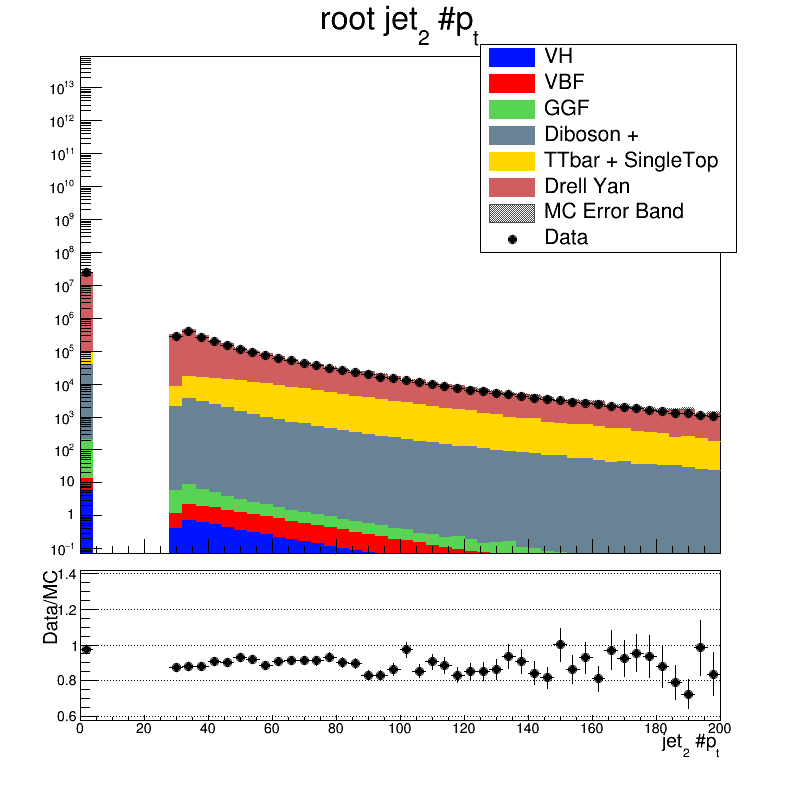
\includegraphics[width=0.32\linewidth]{figures/event_sel/jet2_pt_root.png}
%   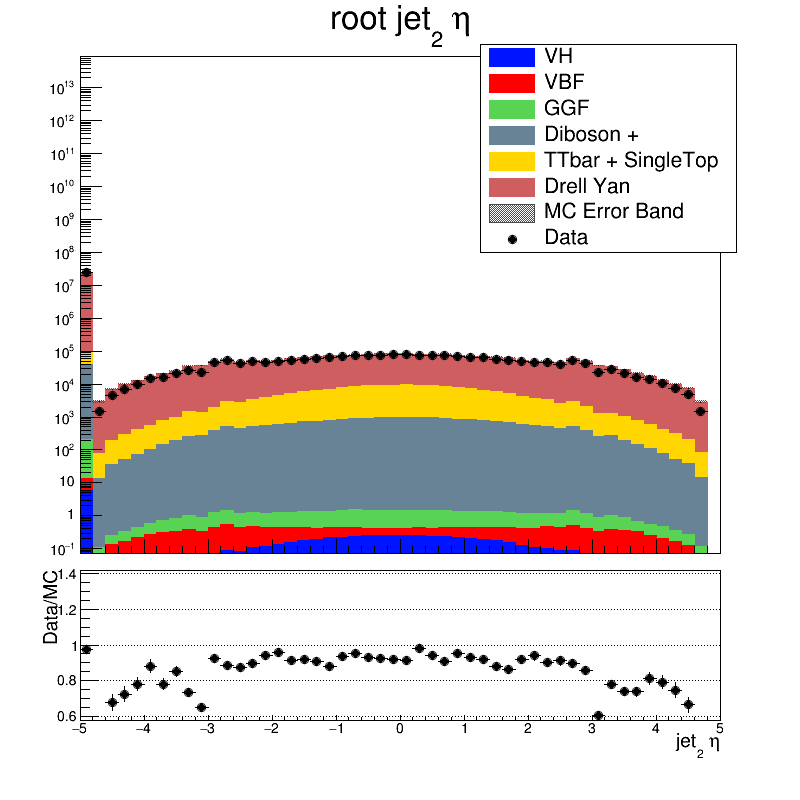
\includegraphics[width=0.32\linewidth]{figures/event_sel/jet2_eta_root.png}
%   \caption
%    {Validation of jet-related variables.}
%   \label{fig:valid_jets}
% \end{figure}



